\chapter{The Case}
%Development
Since no library with Android support currently exist it was decided to use the Motej library as a core for further development.

\section{Introduction}
At the time of writing no research has been done on using motion game controllers as peripherals in a smart-phone based bio-feedback system. In order to answer the research questions posed in this report it will be necessary to create a simple but working prototype of the aforementioned system. The equipment used to realize the system will be a rooted HTC Desire HD \cite{desireHdSpecs} running CyanogenMod 7 and Wii Remotes with the Motion Plus extension. The application will be created using the Android SDK, Java and the Motej library.

%Write about why we chose motej?

\section{Software Architecture}
In this section contains an explination and documentation of the various software architectural choices.

The two main focuses when creating the architecture was \emph{modifiability} and \emph{usability}. Modifiability was important to insure the ability to replace the Wii remote with other senors without major changes in the source code. Though the main goal of this project does not include the creation of a complex graphical user interface, usability was still considered a priority for the source code to be reused in future work. 

\subsection{Architectural Patterns}
\subsubsection{Event-driven architecture}
Event-driven architecture is an architectural pattern that focuses on the creation and cosumption of events. The event emitters creates new events and pushes them to the event consumers. The event consumers uses the events to produce some reaction. Because the event emitter does not directly speak with the event consumers this pattern makes the different components very loosely coupled.

In our case the event emitters will be the motej and motejx libraries. These classes will handle the connection to the Wii remote and the MotionPlus extension and create events when it receives new date from the Wii remote or its extensions. The event consumers will be the models that change the state in accordance to the received events containing the sensor data. Using this pattern the models are not concerned with the way the event emittors are implemented or what kind of sensors they connect to as long as the events emitted are on the same form.

Fortunatly Motej already implemented the event-driven architecture so there was no need to modify the library in this aspect.

\begin{lstlisting}
//Example of event-driven architecture using 
//java.swing.event.EventListenerList and 
//java.util.EventListener

//Event emittor (parts from the Mote class)
EventListenerList listenerList = new EventListenerList();
...
public void addAcceleromterListener(AcceleromterListener<Mote> listener) {
	listenerList.add(AccelertomerListener.class, listener);
}
...
protected void fireAccelerometerEvent(float x, float y, float z) {
	AccelerometerListener<Mote>[] listeners = listenerList
			.getListeners(AccelerometerListener.class);
	AccelerometerEvent<Mote> evt = 
		new AccelerometerEvent<Mote>(this, x, y, z);
	for (AccelerometerListener<Mote> l : listeners) {
		l.accelerometerChanged(evt);
	}
}

//Interface for the listeners (event consumers)
public interface AccelerometerListener<T> extends EventListener {

	public void accelerometerChanged(AccelerometerEvent<T> evt);

}

//Event consumer - example
public class Example implements AccelerometerListener<Mote> {
	...
	public void acceleromterChanged(AcceleromterEvent<Mote> evt){
		//Events are consumed and handled here
	}
}
\end{lstlisting}

\subsubsection{Model View Controller}
In the model view controller pattern the code is separated into three main components (see figure~\ref{fig:mvc}): model, view and controller. The view handles the graphical user interface and its logic displaying the model to the user. The controller updates the model. The model holds the information or state of the application, which is displayed to the user through the model. This setup gives the users the mental model that they are interacting with the model directly.

\begin{figure}[h!]
  \centering
    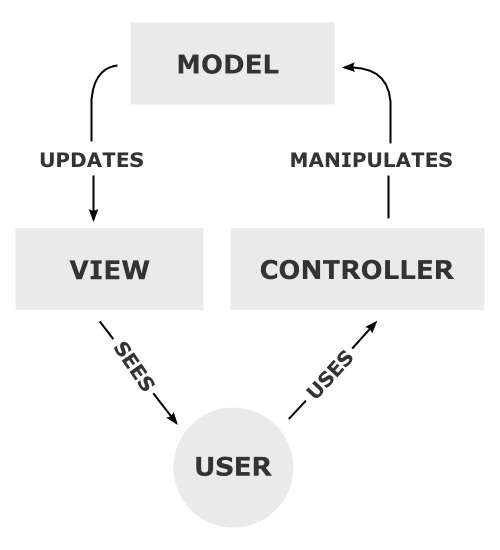
\includegraphics[width=.80\textwidth]{mvc.png}
    \caption{\footnotesize Model-View-Controller pattern}
    \label{fig:mvc}
\end{figure}

Using the model view controller pattern we can easily change the look and feel of the graphical user interface without interfering with how the model is updated. This gives a lot of freedom to continuously modify and improve the graphical user interface during the development of the application. 

\subsection{Package structure}
Using the discussed patterns as a basis, the following package diagram shown in figure~\ref{fig:packageDiagram}. 

\begin{figure}[h!]
  \centering
    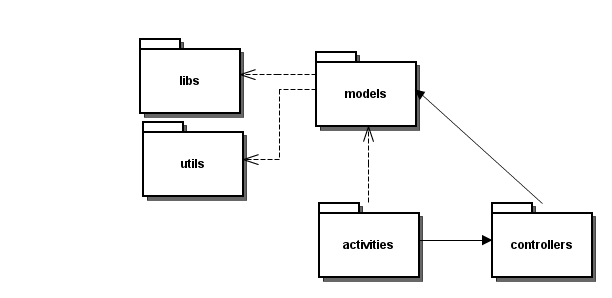
\includegraphics[width=.80\textwidth]{packageDiagram.png}
    \caption{\footnotesize Package diagram}
    \label{fig:packageDiagram}
\end{figure}

\begin{description}
	\item[libs] Contains the library classes used by the project. Currently only contains the java.swing.event.EventListenerList which is used by Motej and Motejx. This class is not included in the standard android packages because swing is not part of android.
	\item[utils] The modified Motej library, our implementation of the MadgwickAHRS algorithm and other help classes resides here. The application uses these classes to update the current state of the Wii remote. 
	\item[modles] Classes holding the state of the Wii remote are contained here.
	\item[activites] Holds the Android activitiy classes.
	\item[controller] Controller classes for interacting with the model are put here.
\end{description}

\section{Limitations}
%Se på dette avsnittet knut. Tror hele må skriver på nytt hvor avsnittene under er merget og forklart bedre
The majority of Android devices have built-in Bluetooth cards, but the current Android SDK does not offer low level support for the Bluetooth stack, including L2CAP. This constraint can be bypassed on some devices by using reflection to access the socket constructor\cite{l2capHtc}. Access could also be gained through using the Android NDK (Native Develeoper Kit) but this is outside of our scope. Due to L2CAP not being official supported, certain vendors of Android devices have removed the L2CAP protocols completely, meaning that it would be impossible to use their Android OS to connect to the Wii Remote. Therefore the Android OS on the HTC Desire HD was altered to run with CyanogenMod 7 instead of the default HTC Sense.

Motej uses the BlueCove library as a multi-platform interface to the Bluetooth stack. Unfortunately, BlueCove does not support the Android OS. Android comes with its own Bluetooth API, the Android Bluetooth API. This means that the library will have to be re-written to work on the Android OS and support for the MotionPlus will have to be implemented. WiiMoteLib\cite{wiiMoteLib} is a C\# library which has support for the MotionPlus, by looking at the solutions in this library it should reduce the time required to implement MotionPlus support for the Motej library.

\section{Motej on Android}
For Motej to work on Android the BlueCove library has to be replaced with the Android Bluetooth API. This presents a major problem. Wii  remotes uses the low level Bluetooth protocol L2CAP to connect to different platforms. As of Android version 4.1, Jelly Bean, \cite{jellyBean} there is no official support for L2CAP. Android only has full support for the higher level protocol \emph{radio frequency communication} (RFCOMM). RFCOMM is built on top of the L2CAP protocol and provides serial port emulation. 

Though the L2CAP is not directly supported through the Android Bluetooth API it is possible to create an L2CAP socket using a technique called reflection.

\begin{lstlisting}
Class<BluetoothSocket> cls = BluetoothSocket.class;
Constructor<BluetoothSocket> constructor = cls.getDeclaredConstructor(
		int.class, int.class, boolean.class, boolean.class,
		BluetoothDevice.class, int.class, ParcelUuid.class);

int type = 3, fd = -1, port = 0x13;
boolean auth = false, encrypt = false;
// Get some device
BluetoothDevice device = getBluetoothDevice();
ParcelUuid uuid = null;

/* type    - Type of socket (3 for L2CAP)
 * fd      - File descriptor (-1 for new socket)
 * auth    - Require authenticaton
 * encrypt - Require encrypted connection
 * port    - Remote port
 * uuid	   - SDP UUID
 */
// This will crate an L2CAP socket on port 0x13
BluetoothSocket socket = constructor.newInstance(type, fd, auth,
		encrypt, device, port, uuid);
\end{lstlisting}

This method has limitations. Because there is no official support for L2CAP in Android, many vendors roms will throw errors when trying to Bluetooth devices this way. Major vendors such as HTC and Samusng does, as of now, not support L2CAP connections.

\section{Motion Plus Support}
Motej has support for most of the common extensions for the Wii remote. Unfortunately Motion Plus is not one of the supported extensions. Motion Plus was implemented using the already existing extension structure of the Motej library.

Information on how to parse the incoming bytes from the Wii remote was found on the WiiBrew wiki \cite{wiiBrew}. The date format is shown in figure~\ref{fig:motionPlusDataFormat}.

\begin{figure}[h!]
  \centering
    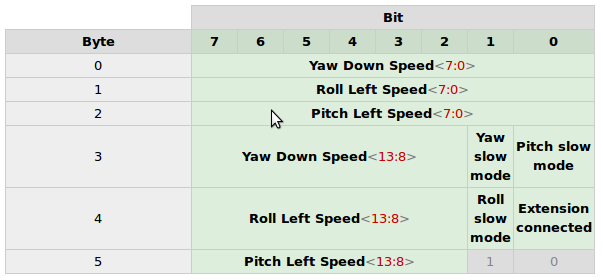
\includegraphics[width=.80\textwidth]{motionPlusDataFormat.png}
    \caption{\footnotesize Motion Plus data gyroscope data format}
    \label{fig:motionPlusDataFormat}
\end{figure}

\begin{lstlisting}
boolean yawFast = ((extensionData[3] & 0x02) >> 1) == 0;
boolean rollFast = ((extensionData[4] & 0x02) >> 1) == 0;
boolean pitchFast = ((extensionData[3] & 0x01) >> 0) == 0;

float yaw = 
	(extensionData[0] & 0xff | (extensionData[3] & 0xfc) << 6);
float roll = 
	(extensionData[1] & 0xff | (extensionData[4] & 0xfc) << 6);
float pitch = 
	(extensionData[2] & 0xff | (extensionData[5] & 0xfc) << 6);
\end{lstlisting}

An additional class was added for manual calibration of the gyroscope. There is calibration data stored in the Wii remote memory, but WiiBrew states that how to use these data for calibration is still unknown. Some suggestions on how to use the data exist, however the calibrated values are not very accurate compared to the manual calibration method. During manual calibration it is required that the Wii remote is kept still. The calibration takes less than 1 second.


When implementing Motion Plus support, another weakness in the Motej library was discovered. After the Motion Plus extension has been connected to the Wii remote, the new data is not sent automatically. To receive the data, the report mode has to be changed. The report mode tells the Wii remote what data to send back to the device it is conneted to. To change the report mode you have to send a some specific bytes to the Wii remote. This functionality is already implemented in Motej, however the library did not check for the message to be received by the Wii remote before allowing new commands to be sent. Because of this, changing the report mode right after initializing the extension was not detected by the Wii remote. 